\section{Introduzione}
%perché, obiettivi, vantaggi...
Nella seconda parte viene descritta l'estensione del progetto iniziale a comprendere un dispositivo di supporto alla proiezione che funzioni out-of-the-box; un Raspberry Pi Zero W facilmente trasportabile e con tempi di boot ridotti.\\
In un tipico utilizzo basterà avviare il mini computer collegandolo ad un power bank, e dopo la sequenza di avvio, il PDF per la presentazione sarà già pronto per essere discusso, mentre il controllo delle slide avverrà tramite smartphone collegato ad un'applicazione web.\\

\section{Panoramica e utilizzo del sistema}
Descriviamo il funzionamento del sistema distinguendo tra due utilizzi principali: un utilizzo wireless, come vera e propria estensione della prima parte del progetto, il Wireless Projector, e un utilizzo wired.\\
In entrambi i setup il Raspberry Pi Zero W è headless e alimentato da un power bank con capacità di 10.000 mAh,  più che sufficiente a coprire l'intervallo temporale occupato da una classica presentazione o lezione.

\paragraph{Uso wireless}

In questo setup, il laptop è sostituito dal Raspberry Pi Zero W su cui è installato e configurato x11vnc così come descritto nella sezione "Configurazione del server - GNU/Linux".\\
Dall'altra parte è necessario che sia presente e correttamente configurato un Raspberry Pi 2 Wireless Projector che accetti la richiesta di connessione VNC in entrata.

\begin{figure}[h!]
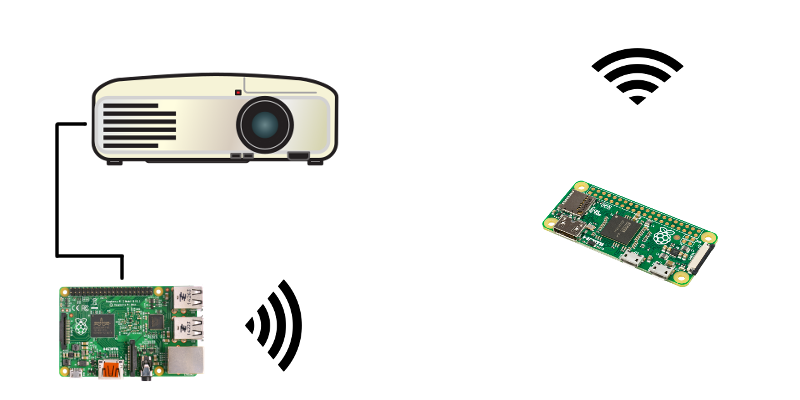
\includegraphics[width=12cm, height=6cm]{../img/setup-with-pizero}
\centering
\caption{VNC on the GO: panoramica del setup con Raspberry Pi ZeroW}
\end{figure}

\paragraph{Uso wired}
Il Raspberry Pi Zero W è collegato al proiettore via cavo HDMI o VGA tramite adattatore, secondo la disponibilità di porte del proiettore stesso.
Questo consente di utilizzare le funzionalità sviluppate nell'estensione anche nei casi in cui si disponga unicamente di proiettori tradizionali.

\section{Configurazione del sistema} %% lo script di avvio...per vnc, e webapp

È stata predisposta una cartella /home/pi/Presentation destinata a contenere i documenti PDF da visualizzare durante una sessione di proiezione, la presentazione di standard aperta all'avvio è denominata "default.pdf", da questa successivamente si potranno aprire le altre eventuali presentazioni presenti nella directory.\\
Si prevede che il caricamento dei file su Raspberry Pi Zero W possa avvenire in vari modi, ad esempio tramite chiavetta USB, lettore di SD card o protocollo SCP.\\
Sul sistema si trova uno script (/home/pi/startup.sh) che chiamato all'avvio tramite .desktop file ha tre compiti: avviare la connessione VNC (per uso wireless), eseguire l'applicazione web Piremote, eseguire il programma Evince con la presentazione base.\\

Piremote, che viene eseguita dallo script, è contenuta di default in /home/pi.\\
\noindent Di seguito sono riportati i dettagli della configurazione:\\

\begin{lstlisting}
cd /home/pi/.config
mkdir autostart
cd autostart
nano startup.desktop
\end{lstlisting}

\noindent Scrivere nel file di configurazione (apportando eventuali modifiche):

\begin{lstlisting}
[Desktop Entry]
Type=Application
Name=Startup
Exec=lxterminal -e /home/pi/startup.sh
Terminal=true
\end{lstlisting}

\begin{lstlisting}
sudo nano /etc/hosts
>> 192.168.1.73    projector.localdomain        projector
\end{lstlisting}

\noindent Il contenuto dello script startup.sh:
\begin{lstlisting}
#! /bin/bash

x11vnc --connect projector:5500 &
sleep 10s
cd /home/pi/piremote
python -m piremote.main &
sleep 10s
evince /home/pi/Presentation/default.pdf &

\end{lstlisting}

%chmod u+x startup.sh

%N.B.
%L’unica pecca è che uno ha solo 10 secondi per visualizzare l’indirizzo, perché poi il terminale potrebbe venire coperto dal pdf. Potrei aggiungere un’iconcina con qt che visualizzi solo l’indirizzo ma non ho tempo adesso.

La configurazione per uso \textit{wired} è molto simile; l'unica differenza è che non sarà necessario eseguire anche VNC all'avvio.\\
\section{Piremote}
Come visualizzatore di documenti PDF è stato scelto Evince, un programma semplice e leggero disponibile nella distribuzione.
Per controllare la presentazione si è realizzato un semplice controller accessibile attraverso un browser web da un qualsiasi dispositivo mobile (o desktop) collegato alla stessa LAN in cui si trova il Pi Zero W. Con tale applicazione è possibile trasformare il proprio smartphone ad esempio, in un telecomando del tutto simile ad un presenter. \\
L'applicazione è molto semplice e supporta le operazioni di base per il controllo della presentazione: lo scorrimento delle pagine avanti e indietro, l'apertura di un file .pdf a partire da una directory designata (/home/pi/Presentation) e il passaggio a schermo intero nella modalità di presentazione.

Per poter accedere a tutte le funzionalità è necessario inserire nella schermata iniziale un pin o una password per autenticarsi, dopodiché si verrà reindirizzati alla pagina principale.

Piremote è stata rilasciata con licenza MIT ed è disponibile all'indirizzo https://github.com/giulic3/piremote.

\begin{figure}[h!]
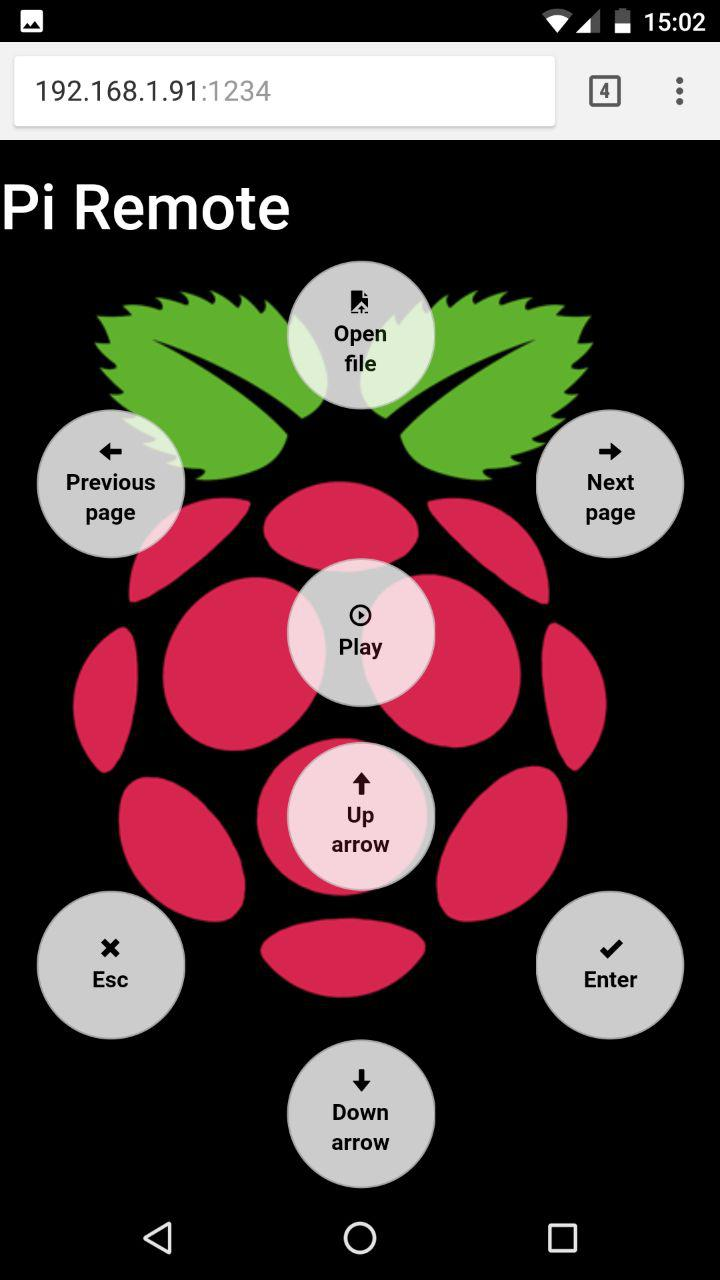
\includegraphics[width=6cm, height=11cm]{../img/main-page}
\centering
\caption{Piremote: pagina principale}
\end{figure}

Dall'alto verso il basso:
il bottone "Open file" consente di aprire un file PDF che si trova all'interno della stessa directory in cui si trova la presentazione corrente;\\
"Previous page" e "Next page" permettono di scorrere le pagine della presentazione corrente;\\
premendo "Play" è possibile passare alla modalità presentazione, a schermo intero;\\
le frecce "Up arrow" e "Down arrow" consentono la navigazione della directory all'apertura di un file;\\
con "Esc" è possibile uscire dalla modalità presentazione;\\
con "Enter" si seleziona un file PDF.\\
